\documentclass{beamer}
\usetheme{Berlin}
\usepackage{graphicx}
\usepackage{subfig}

% Naslovnica
\title{Napredna računalniška orodja - domača naloga 1}
\author{Jacopo Komic}
\institute{Univerza v Ljubljani - Fakulteta za strojništvo}
\date{23. oktober 2023}

\begin{document}

% ------------------------------------------------------------ slide 1
\begin{frame}
\begin{center}

\includegraphics[width = 0.2 \linewidth]{logotip.jpg}  
\end{center}
\titlepage
\end{frame}

% ------------------------------------------------------------ slide 2
\begin{frame}
\frametitle{Kazalo}
\tableofcontents
\end{frame}

% ------------------------------------------------------------ slide 3
\section{Cilj}
\begin{frame}
\frametitle{Cilj}

\begin{itemize}
  \item izračunali bomo približno vrednost $\pi$ po metodi Monte Carlo\pause
  \item primerjali ploščino kroga in njemu očrtanega kvadrata\pause
  \item pomagali si z naključno generiranimi točkami
\end{itemize}

\end{frame}

% ------------------------------------------------------------ slide 4
\section{Funkcijska datoteka}
\begin{frame}
\frametitle{Funkcijska datoteka}

\begin{figure}
  \centering
  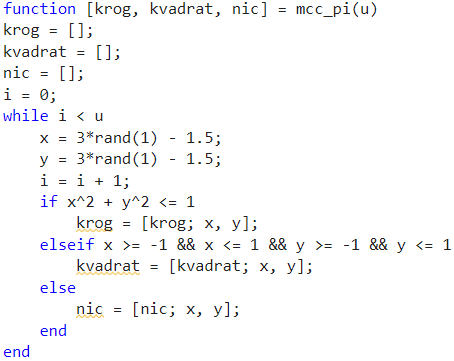
\includegraphics[width = 0.6 \linewidth]{slika_1.png}
  \caption{Prikaz funkcijske datoteke.}
\end{figure}

\end{frame}

% ------------------------------------------------------------ slide 5
\section{Programska datoteka}
\begin{frame}
\frametitle{Programska datoteka}

\begin{figure}
  \centering
  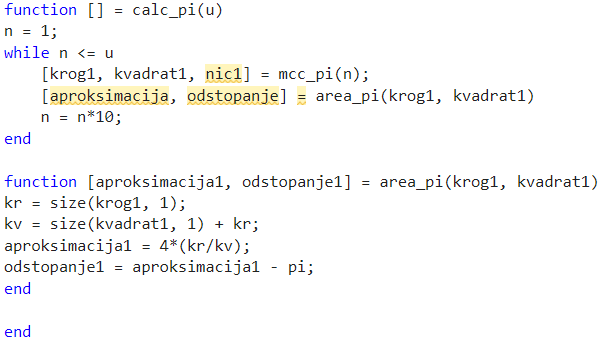
\includegraphics[width = 0.6 \linewidth]{slika_2.png}
  \caption{Prikaz programske datoteke.}
\end{figure}

\end{frame}

% ------------------------------------------------------------ slide 6
\section{Anonimna funkcija in koda za vizualizacijo}
\begin{frame}
\frametitle{Anonimna funkcija in koda za vizualizacijo}

\begin{figure}
  \subfloat{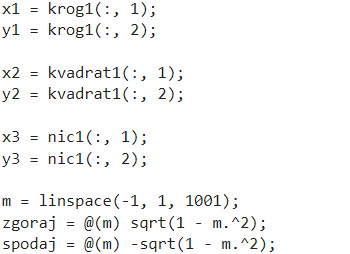
\includegraphics[width = 0.45 \linewidth]{slika_3.png}}
  \subfloat{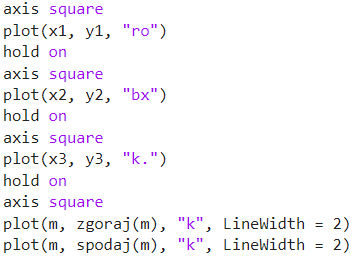
\includegraphics[width = 0.45 \linewidth]{slika_4.png}}
  \caption{Prikaz anonimnih funkcij in kode za vizualizacijo.}
\end{figure}

\end{frame}

% ------------------------------------------------------------ slide 7
\section{Vizualizacija}
\begin{frame}
\frametitle{Vizualizacija - 100 točk}

\begin{figure}
  \centering
  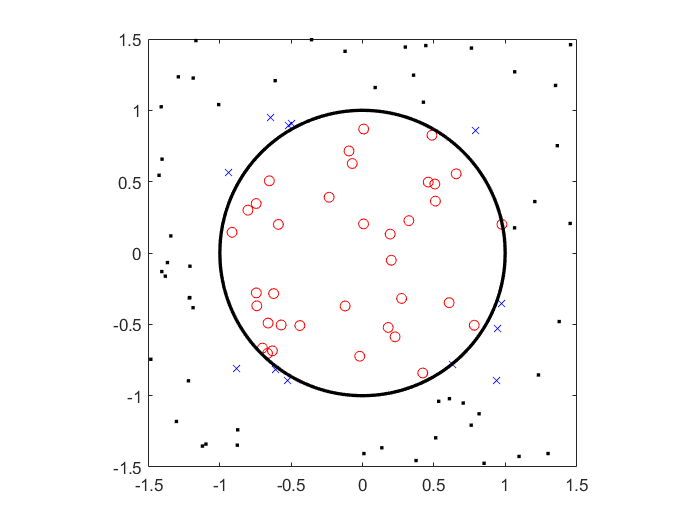
\includegraphics[width = 0.6 \linewidth]{100.png}
\end{figure}
\centering
aproksimacija = 3, odstopanje = -0.1416

\end{frame}

% ------------------------------------------------------------ slide 8
\begin{frame}
\frametitle{Vizualizacija - 1000 točk}

\begin{figure}
  \centering
  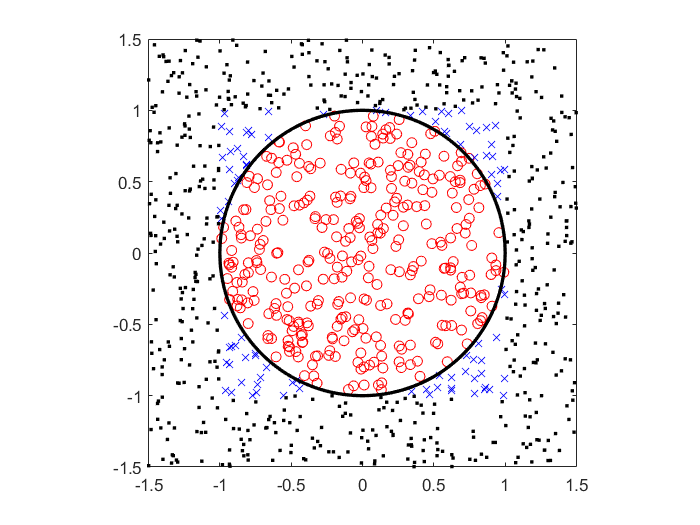
\includegraphics[width = 0.6 \linewidth]{1000.png}
\end{figure}
\centering
aproksimacija = 3.1422, odstopanje = 5.9849e-04

\end{frame}

% ------------------------------------------------------------ slide 9
\begin{frame}
\frametitle{Vizualizacija - 10000 točk}

\begin{figure}
  \centering
  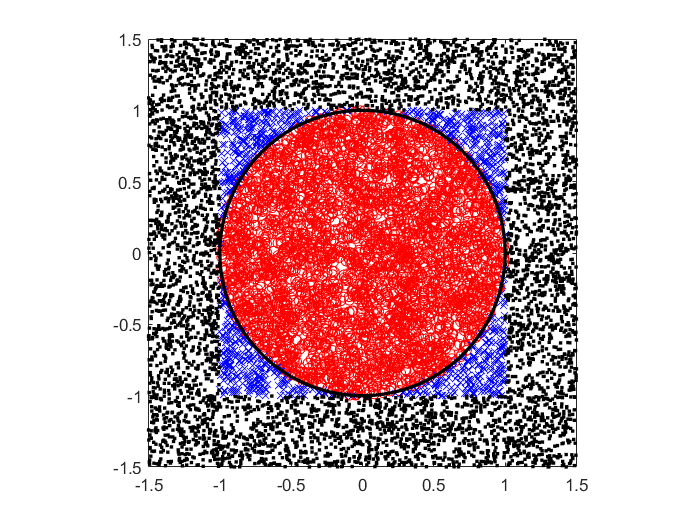
\includegraphics[width = 0.6 \linewidth]{10000.png}
\end{figure}
\centering
aproksimacija = 3.1555, odstopanje = 0.0140

\end{frame}

% ------------------------------------------------------------ slide 10
\section{Zaključek}
\begin{frame}
\frametitle{Zaključek}

\begin{itemize}
  \item metoda je kar natančna
  \item pri izračunu s 1000 točkami se nam je "posrečilo" in smo dobili celo boljšo aproksimacijo kot z 10000 točkami
\end{itemize}

\end{frame}

\end{document}